%%%%%%%%%%%%%%%%%%%%%%%%%%%%%%%%%%%%%%%%%%%%%%%%%%%%%%%%%%%%%%%%%%%%%%%%%%%%%%
%
% Section file included in main project file using \input{}
%
% Assumes that LaTeX2e macros and packages defined in cg_comp.sty are
%   available
%
%%%%%%%%%%%%%%%%%%%%%%%%%%%%%%%%%%%%%%%%%%%%%%%%%%%%%%%%%%%%%%%%%%%%%%%%%%%%%%

 \section{Classical Guitar Compensation\label{sct:comp}}

 \begin{equation}\label{eqn:error_comp}
\Delta \nu_n \approx \frac{1200}{\ln(2)}\, \left[ \gamma_n \left(B_0 - \frac{\Delta S}{X_0}\right) + \frac{\Delta N}{X_0} + \half\, \kappa\, Q_n \right]\, .
 \end{equation}

\red{Strategy: Use $\Delta S$ to compensate for bending stiffness, and $\Delta N$ to compensate for tension increases arising from fretting. Doing so predicts that $\Delta S \approx 3$~mm for the Alhambra 8P with light-tension strings, or about twice the saddle setback that is actually manufactured.}

 \begin{figure}
  \centering
  \begin{subfigure}[b]{0.45\textwidth}
   \centering
   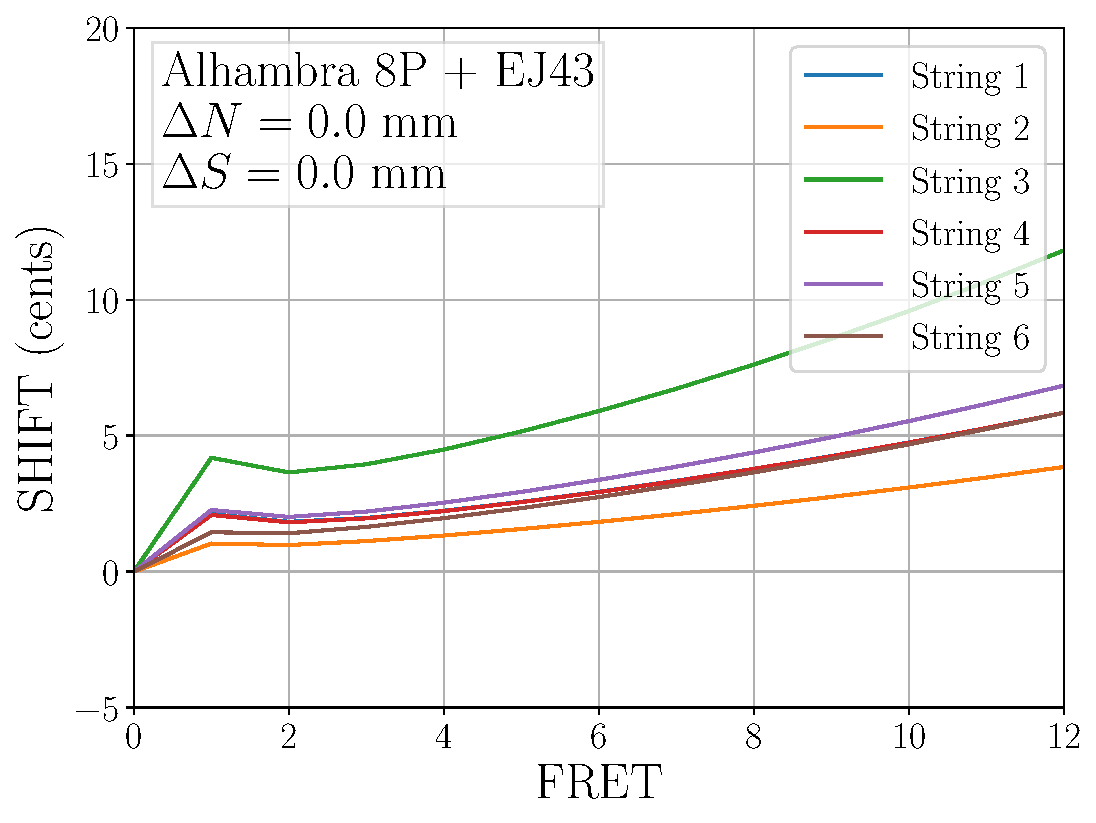
\includegraphics[width=3.25in]{figures/shift_alhambra8p_ej43_null}
   \caption{Uncompensated}
   \label{fig:shift_alhambra8p_ej43_null}
  \end{subfigure}
  \hspace{0.25in}
  \begin{subfigure}[b]{0.45\textwidth}
   \centering
   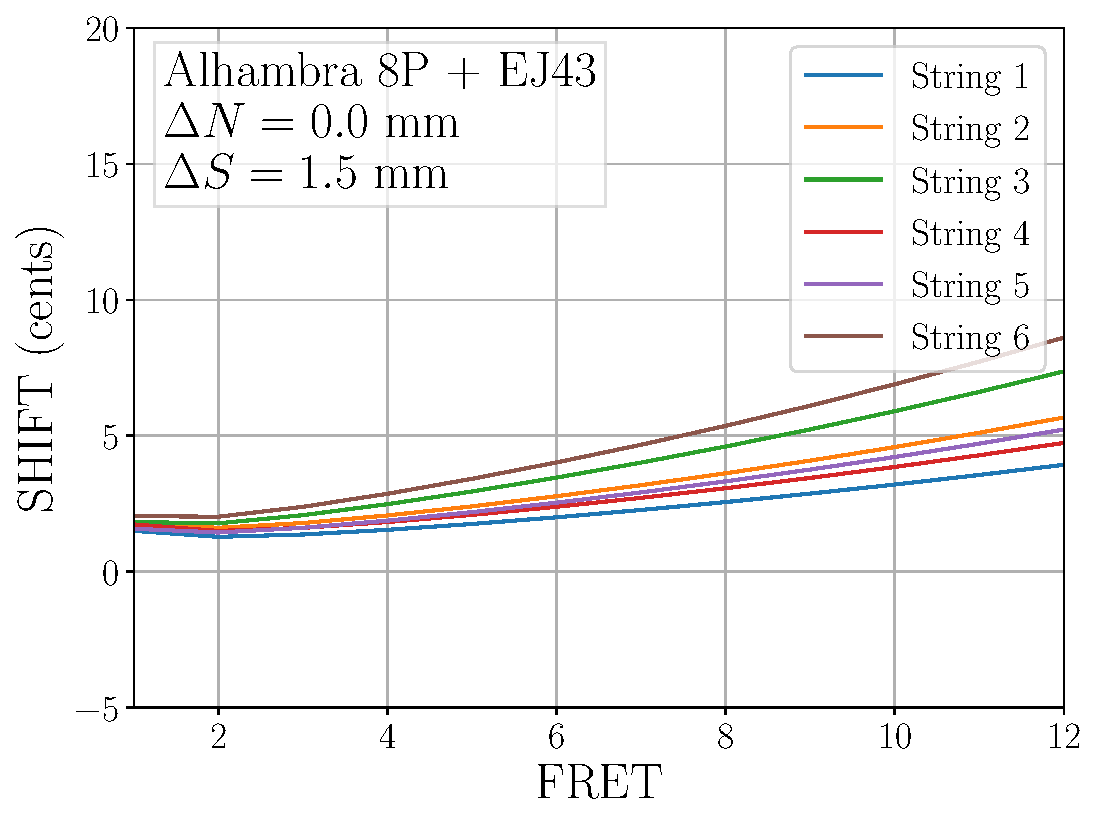
\includegraphics[width=3.25in]{figures/shift_alhambra8p_ej43_factory}
   \caption{Factory guitar}
   \label{fig:shift_alhambra8p_ej43_factory}
  \end{subfigure}
  \par\vspace{0.25in}
  \begin{subfigure}[b]{0.45\textwidth}
   \centering
   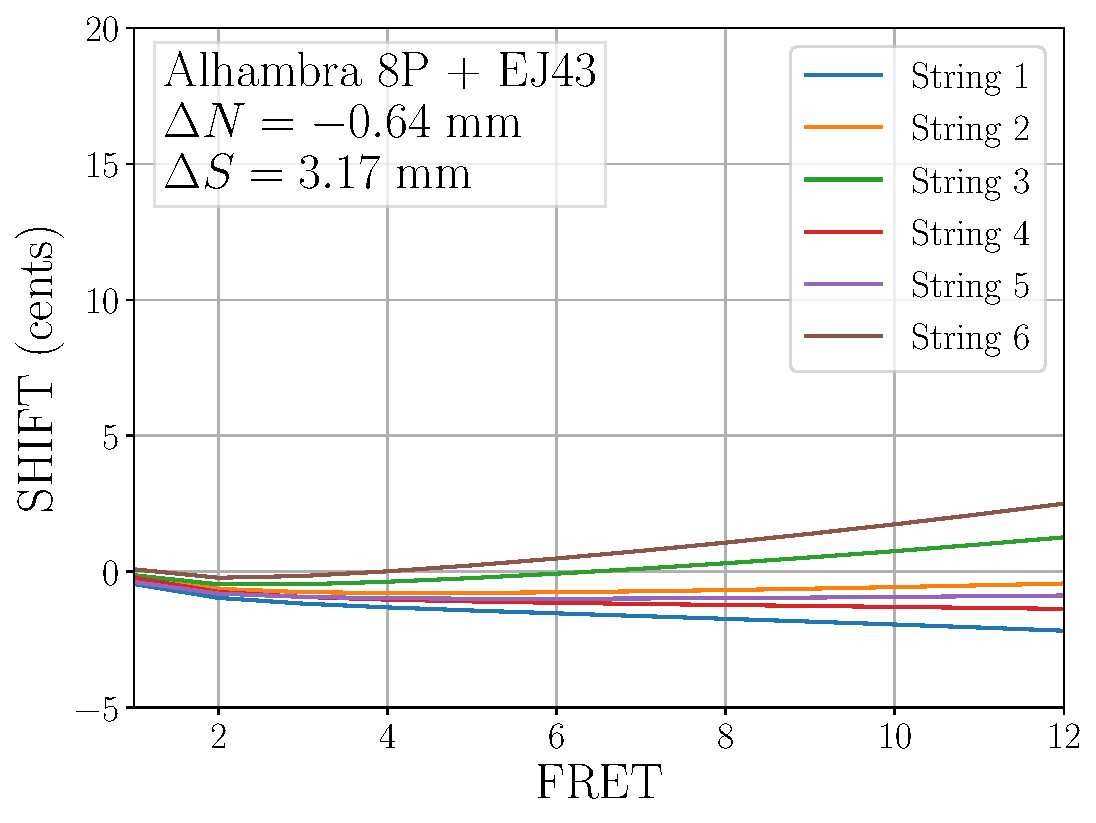
\includegraphics[width=3.25in]{figures/shift_alhambra8p_ej43_avg}
   \caption{Average compensation}
   \label{fig:shift_alhambra8p_ej43_avg}
  \end{subfigure}
  \hspace{0.25in}
  \begin{subfigure}[b]{0.45\textwidth}
   \centering
   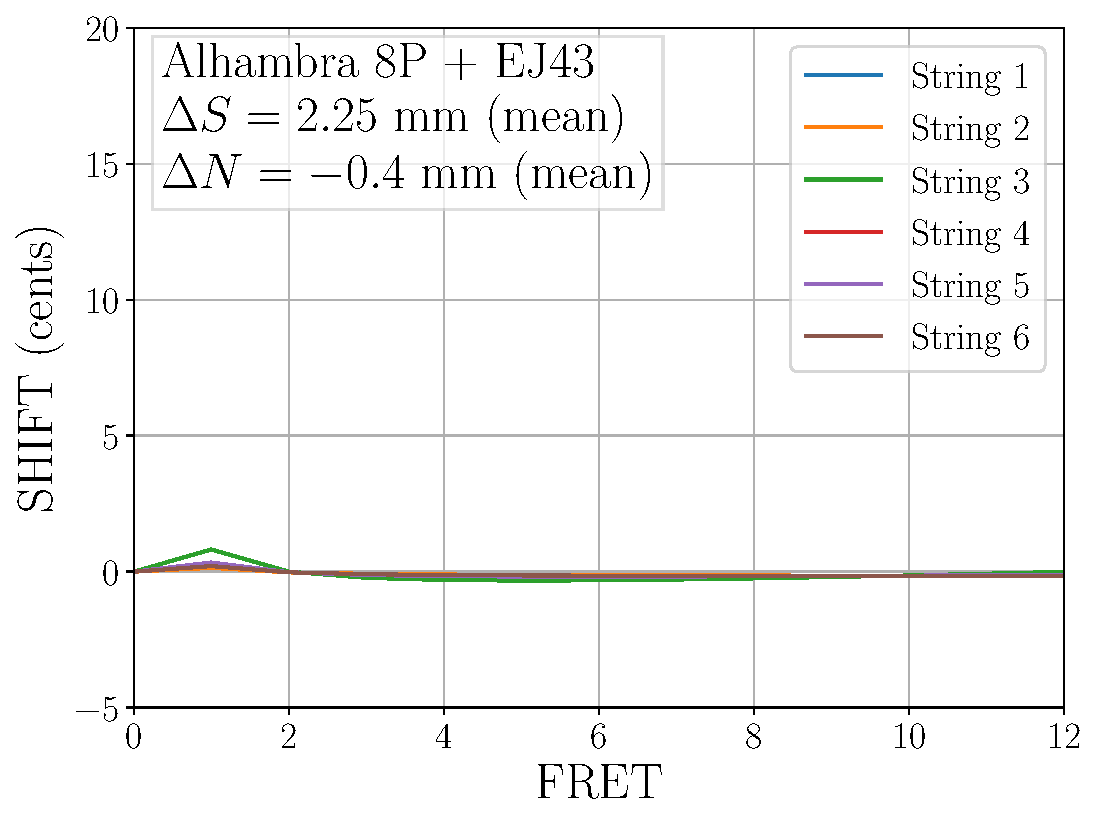
\includegraphics[width=3.25in]{figures/shift_alhambra8p_ej43_full}
   \caption{Full compensation \red{(currently only for string 4)}}
   \label{fig:shift_alhambra8p_ej43_full}
  \end{subfigure}
  \caption{\label{fig:compensation} Frequency shift (in cents) for an Alhambra 8P guitar with D'Addario Pro-Arte Nylon Classical Guitar Strings -- Light Tension (EJ43). Four different strategies of saddle and nut compensation are illustrated.}
 \end{figure}


